\documentclass[12pt, a4paper]{article}
%\usepackage{helvet}
%\renewcommand{\familydefault}{\sfdefault}
\usepackage{amssymb}
\usepackage{amsmath}
\usepackage{tikz} 
\title{Chapter 0}
\author{Maciej Harbuz}

\begin{document}

\maketitle

\section{Exercises}

\begin{enumerate}

    \item[0.1]
Examine the following formal descriptions of sets so that you understand which members they contain. Write a short informal English description of each set.
\begin{enumerate}

\item 
$\{1, 3, 5, 7, \ldots \}$

Set of odd, natural numbers.
\item 
$\{x \ldots, -4, -2, 0, 2, 4 \ldots \}$

Set of even, integer numbers.
\item 
$\{n \mid n = 2m \text{for some \textit{m}} \in \mathbb{N} \}$

Set of even, natural numbers.
\item 
$\{n \mid n = 2m \text{for some \textit{m}} \in \mathbb{N}, \text{and} n = 3k \text{for some} k \in \mathbb{N} \}$

Set of even, natural numbers that are also multiples of 3.
\item 
$\{w \mid w  \text{is a string of \textit{0s} and \textit{1s} and \textit{w} equals the reverse of} w\}$

Set of strings of 0s and 1s that are palindroms 
\item $\{ n \mid n \text{is an integer and}  n = n+1\}$

Set of integers that are equal to their successor which is \textit{empty set}
\end{enumerate}

    \item[0.2]
Write  formal descriptions  of the following sets.

\begin{enumerate}
\item The set containing the numbers 1, 10, and 100

    $\{1, 10, 100\}$
\item The set containing all integers that are greater than 5
    
    $\{n \mid n > 5, n \in \mathbb{Z}\}$
\item  The set containing all natural numbers that are less than 5:

    $\{n \mid n < 5, n \in \mathbb{N}\}$
\item The set containing the string "aba":

    $\{"aba"\}$
\item The set containing the empty string:

    $\{\epsilon\}$
\item The set containing nothing at all:

    $\emptyset$
\end{enumerate}

    \item[0.3]

Let $A$ be the set $\{x,y,z\}$ and $B$ be the set $\{x,y\}$
\begin{enumerate}
\item Is $A$ a subset of $B$? ($A \subseteq B$) 

    No, $A$ is not a subset of $B$
\item Is $B$ a subset of $A$? ($B \subseteq A$) 

    Yes, $B$ is a subset of $A$
\item What is the union of $A$ and $B$? ($A \cup B$) 

    $\{x,y,z\} = A$
\item What is the intersection of $A$ and $B$? ($A \cap B$) 

    $\{x,y\} = B$
\item What is the cross product $A$ and $B$? ($A \times B$) 

    $\{(x,x), (x,y), (y,x), (y,y), (z,x), (z,y)\}$

\item What is the power set of $B$? 

$\mathcal{P}(B) = \{\emptyset, \{x\}, \{y\}, \{x,y\}\}$
\end{enumerate}

    \item[0.4]
If $A$ has  $a$  elements and  $B$  has  $b$  elements, how many elements are in  $A \times B$? 
Explain your answer.

The cross product of two sets $A$ and $B$ is the set of all possible ordered pairs of elements from $A$ and $B$. If $A$ has $a$ elements and $B$ has $b$ elements, then the cross product $A \times B$ will have $a \cdot b$ elements.

    \item[0.5]
If $C$ is a set with $c$ elements, how many elements are in the power set of $C$? 
Explain your answer.

The power set of a set $C$ is the set of all possible subsets of $C$. If $C$ has $c$ elements, then the power set of $C$ will have $2^c$ elements. Thats  because every element can be present or absent in every subset, so there are $2^c$ possible combinations of elements in the power set of $C$.

    \item[0.6]
Let X be the set $\{1, 2, 3, 4, 5\}$ and $Y$ be the set $\{6, 7, 8, 9, 10\}$. The unary function $f: X \to Y$ and the binary function $g: X \times Y \to Y$ are described in the following tables.

\begin{tabular}{ c | c }
    n & f(n) \\
    \hline
    1 & 6 \\
    2 & 7 \\
    3 & 6 \\
    4 & 7 \\
    5 & 6 \\
\end{tabular}
\begin{tabular}{ c | c | c | c | c | c }
    g(x,y) & 6 & 7 & 8 & 9 & 10 \\
    \hline
    1 & 10 & 10 & 10 & 10 & 10 \\
    2 & 7 & 8 & 9 & 10 & 6 \\
    3 & 7 & 7 & 8 & 8 & 9 \\
    4 & 9 & 8 & 7 & 6 & 10 \\
    5 & 6 & 6 & 6 & 6 & 6 \\
\end{tabular}
\begin{enumerate}
\item What is the value of f(2)? 

    $f(2) = 7$
\item What are the range and domain of f?
\begin{itemize}
    \item Range: $\{6, 7\}$
    \item Domain: $\{1, 2, 3, 4, 5\}$
\end{itemize}

\item What is the value of $g(2, 10)$?

    $g(2, 10) = 6$
\item What are the range and domain of g?
\begin{itemize}
    \item Range: $\{6, 7, 8, 9, 10\}$
    \item Domain: $\{1, 2, 3, 4, 5\}$
\end{itemize}

\item What is the value of $g(4, f(4))$?

    $g(4, f(4)) = 8$
\end{enumerate}

    \item[0.7]
For each part, give a relation that satisfies the condition.
\begin{enumerate}
    \item  Reflexive
    \footnote{Reflexive relation $R$ is when $\forall a \in A, (a, a) \in R$} and symmetric
    \footnote{Symmetric relation $R$ is when $\forall a, b \in A, (a, b) \in R \implies (b, a) \in R$} but not transitive.
    \item  Reflexive and transitive
    \footnote{Transitive relation $R$ is when $\forall a, b, c \in A, (a, b) \in R \land (b, c) \in R \implies (a, c) \in R$} but not symmetric.
    \item  Symmetric and transitive but not reflexive.
\end{enumerate}

\begin{enumerate}

    \item Reflexive and symmetric but not transitive example is be coworker relation on the set of people (let's assume that everybody is a coworker with themselves)
    \item Reflexive and transitive but not symmetric example is greater than or equal to relation on the set of natural numbers
    \item Symmetric and transitive but not reflexive example is the relation "is a sibling of" on the set of people
\end{enumerate}

    \item[0.8]
Consider the undirected graph $G = (V, E)$ where $V$, the set of nodes, is $\{1, 2, 3, 4\}$ and $E$, the set of edges, is $\{\{1, 2\}, \{2, 3\}, \{1, 3\}, \{2, 4\}, \{1, 4\}\}$. Draw the graph $G$. What are the degrees of each node? Indicate a path from node 3 to node 4 on your drawing of $G$.

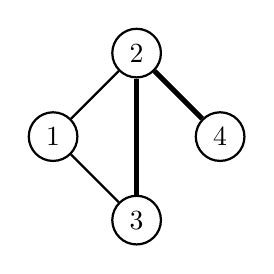
\begin{tikzpicture}[node distance={15mm}, thick, main/.style = {draw, circle}] 
\node[main] (1) {$1$}; 
\node[main] (2) [above right of=1] {$2$}; 
\node[main] (3) [below right of=1] {$3$}; 
\node[main] (4) [above right of=3] {$4$}; 
\draw[-] (1) -- (2); 
\draw[-] (1) -- (3); 
\draw[-, line width=1.8pt] (2) -- (3); 
\draw[-, line width=1.8pt] (2) -- (4); 
\end{tikzpicture} 

    \item[0.9]
Write a formal description of the following graph.

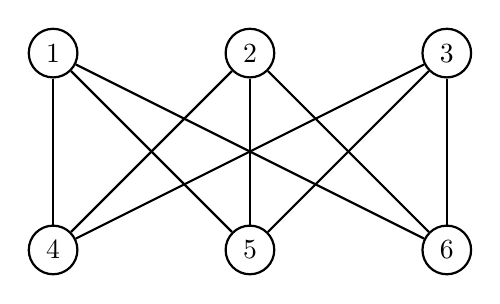
\begin{tikzpicture}[node distance={25mm}, thick, main/.style = {draw, circle}] 
    \node[main] (1) {$1$}; 
    \node[main] (2) [right of=1] {$2$}; 
    \node[main] (3) [right of=2] {$3$}; 
    \node[main] (4) [below of=1] {$4$}; 
    \node[main] (5) [right of=4] {$5$}; 
    \node[main] (6) [right of=5] {$6$}; 
    \draw[-] (1) -- (4); 
    \draw[-] (1) -- (5);
    \draw[-] (1) -- (6);
    \draw[-] (2) -- (4);
    \draw[-] (2) -- (5);
    \draw[-] (2) -- (6); 
    \draw[-] (3) -- (4);
    \draw[-] (3) -- (5);
    \draw[-] (3) -- (6); 
    \end{tikzpicture} 

$G = (V, E)$ where 

$V = \{1, 2, 3, 4, 5, 6\}$ and 

$E = \{\{1, 4\}, \{1, 5\}, \{1, 6\}, \{2, 4\}, \{2, 5\}, \{2, 6\}, \{3, 4\}, \{3, 5\}, \{3, 6\}\}$
\end{enumerate}
\section{Problems}

\begin{enumerate}

    \item[0.10]
Find the error in the following proof that $2 = 1$. 

Consider the equation $a = b$. Multiply both sides by a to obtain 
$a^2 = ab$. 
Subtract 
$b^2$ 
from both sides to get 
$a^2 - b^2 = ab - b^2$
. Now factor each side, 
$(a + b)(a - b) = b(a - b)$
, and divide each side by 
$(a - b)$ 
to get 
$a + b = b$
. Finally, let a and $b$ equal $1$, which shows that $2 = 1$.


We cannot divide each side of equation $(a + b)(a - b) = b(a - b)$ by $(a - b)$ because $a = b$ implies $a - b = 0$ and division by zero is undefined.

    \item[0.11]
Let $S(n) = 1 + 2 + \ldots + n$ be the sum of the first $n$ natural numbers, and let $C(n) = 1^3 + 2^3 + \ldots + n^3$ be the sum of the first n cubes. Prove the following equalities by induction on $n$, to arrive at the curious conclusion that $C(n) = S^2(n)$ for every $n$.

1. $S(n) = \frac{1}{2} n(n+1)$.

\textbf{Basis}
$ S(1) = 1 = \frac{1}{2} 1(1+1)$.

\textbf{Induction step}

$ S(k+1) = S(k) + (k+1) = \frac{1}{2} k(k+1) + (k+1) = \frac{1}{2} (k+1)(k+2)$.

2. $C(n) = \frac{1}{4}(n^4 + 2n^3 + n^2) = \frac{1}{4} n^2(n+1)^2$.

\textbf{Basis}

$ C(1) = 1 = \frac{1}{4} 1^2(1+1)^2$

\textbf{Induction step}

$ C(k+1) = C(k) + (k+1)^3 = \frac{1}{4} k^2(k+1)^2 + (k+1)^3 = \frac{1}{4} (k+1)^2(k+2)^2$.

The induction step is valid for both $S(n)$ and $C(n)$. 

Therefore, $C(n) = S^2(n)$ for every $n$.

$S^2(n)$ is $(\frac{1}{2} n(n+1))^2 = \frac{1}{4} n^2(n+1)^2$ which is equal to $C(n)$.

    \item[0.12]
Find the error in the following proof that all horses are the same color.

\textbf{CLAIM}: In any set of h horses, all horses are the same color.

\textbf{PROOF}: By induction on h.

\textbf{Basis}: 

For $h = 1$. In any set containing just one horse, all horses clearly are the same color.

\textbf{Induction step}

The horse removed in the first step may have a different color than the horse removed in the second step. Therefore, the induction step is invalid.

\item[0.13]
Show that every graph with two or more nodes contains two nodes that have equal degrees.

\item[0.14]
Ramsey's theorem. 

Let $G$ be a graph. A clique in $G$ is a subgraph in which every two nodes are connected by an edge. An anti-clique, also called an independent set, is a subgraph in which every two nodes are not connected by an edge. Show that every graph with $n$ nodes contains either a clique or an anti-clique with at least $\frac{1}{2} log_2(n)$ nodes.


\item[0.15]
Use Theorem 0.25 to derive a formula for calculating the size of the monthly payment for a mortgage in terms of the principal P, the interest rate I, and the number of payments t. Assume that after t payments have been made, the loan amount is reduced to 0. Use the formula to calculate the dollar amount of each monthly payment for a 30-year mortgage with 360 monthly payments on an initial loan amount of \$100,000 with a 5% annual interest rate.


**Theorem 0.25**

$\forall t \geq 0$


$P_t=PM^t-Y\frac{M^t-1}{M-1}$
\end{enumerate}
\end{document}
